\documentclass[11pt]{article}

% template
\usepackage{if69d-template} % Modelo elaborado por Fernando Padilha 

% pacotes
\usepackage[brazil]{babel}
\usepackage[utf8]{inputenc}
\usepackage{graphicx}
\usepackage{amsthm,amsfonts,amsmath}
\usepackage[font=footnotesize,
			labelfont=it,
			labelformat=simple]{subcaption}
\renewcommand\thesubfigure{(\alph{subfigure})}

% capa
\instituicao{Universidade Tecnológica Federal do Paraná -- UTFPR -- Campus Curitiba}
\departamento{Departamento Acadêmico de Eletrônica -- DAELN}
\curso{Curso de Engenharia Eletrônica}
\disciplina{IF69D e OPEET014 –- Processamento Digital de Imagens}
\semestre{2025.2}
\professor{Gustavo B. Borba}

\titulo{Modelo e instruções (título do seu relatório)} % INSIRA AQUI O TÍTULO DO SEU RELATÓRIO

\autor{Nome completo}{RA} %INSIRA SUA IDENTIFICAÇÃO
\autordois{Nome completo}{RA} %INSIRA SUA IDENTIFICAÇÃO
\date{mês.ano} %INSIRA AQUI MÊS E ANO DA ENTREGA


% começo do documento
\begin{document}

\maketitle

\section{Objetivo}

Descrever em poucas palavras o objetivo (enunciado) do trabalho. Exemplo: Apresentar  ao aluno o modelo e instruções para a execução do relatório a ser utilizado nos projetos finais da disciplina IF69D. Um exemplo mais específico: sendo o título ``Filtros Homomórficos'', o objetivo pode ser: Implementar em MATLAB um filtro homomórfico para imagens em níveis de cinza. 


\section{Fundamentação Teórica}

Informações teóricas relevantes a respeito do algoritmo a ser implementado. Descrever a sua aplicação prática e todos os conceitos e informações necessárias para sua compreensão, como, por exemplo,  equações, pseudocódigo, figuras. Citar as referências utilizadas através de um índice como este~\cite{gonzalez:92}.

As equações devem ser citadas no texto e inseridas conforme mostrado a seguir. Exemplo: A relação sinal-ruído de uma imagem pode ser obtida a partir da equação~\ref{eq:snr}~\cite{kwan:99}.

\begin{equation} \label{eq:snr}
SNR_g = \frac{S}{\sigma_b}
\end{equation}

\noindent onde $S$ é a média do sinal e $\sigma_b$ o desvio padrão do ruído no background.

As figuras devem ser citadas e explicadas no texto e inseridas conforme ilustrado a seguir. Todas as figuras devem ter legenda. Exemplo: A imagem da Figura~\ref{fig:lenac} demonstra a aplicação do filtro da mediana 3x3 na imagem~\ref{fig:lenab}, degradada por ruído sal e pimenta, com 5\% de probabilidade para os pixels claros e 5\% de probabilidade para os pixels escuros. A imagem original é mostrada na Figura~\ref{fig:lenaa}.

\begin{figure}[!htb]
	\centering
	\begin{subfigure}[b]{0.3\textwidth}
		\centering
		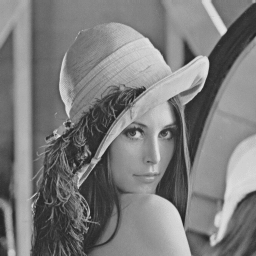
\includegraphics[width=.8\textwidth]{lena}
		\caption{}
		\label{fig:lenaa}
	\end{subfigure}
	\begin{subfigure}[b]{0.3\textwidth}
		\centering
		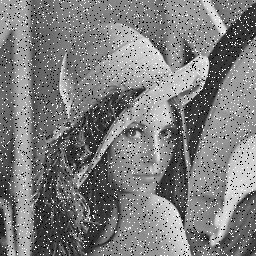
\includegraphics[width=.8\textwidth]{lena_salt}
		\caption{}
		\label{fig:lenab}
	\end{subfigure}
	\begin{subfigure}[b]{0.3\textwidth}
		\centering
		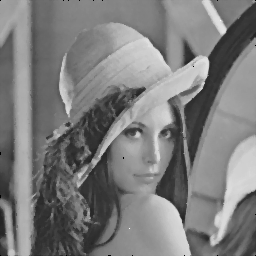
\includegraphics[width=.8\textwidth]{lena_med}
		\caption{}
		\label{fig:lenac}
	\end{subfigure}
	\caption{\subref{fig:lenaa} Imagem Lena original. \subref{fig:lenab} Imagem Lena degradada por ruído sal e pimenta, com 5\% de probabilidade para os pixels claros e 5\% de probabilidade para os pixels escuros. \subref{fig:lenac} Saída do filtro da mediana 3x3.}
	\label{fig:lena}
\end{figure}

As tabelas devem ser citadas e explicadas no texto e inseridas de maneira semelhante às figuras, porém com as legendas no topo. Todas as tabelas devem ter legenda.

\subsection{Mais de um nível}

Havendo sub-itens, estes não devem passar deste nível. Se necessários mais deles, utilizar marcadores como a seguir:

\begin{itemize}
\item \textbf{Fonte, parágrafos, paginação e cabeçalho} \\
Seguir o modelo. Observe que o espaçamento entre as linhas do corpo do texto é simples, e a fonte é Times 11. A paginação utiliza o formato n/m, onde n é a página atual e m número total de páginas. O cabeçalho (\textit{header}) deve conter o título do relatório. Se for um título extenso, escreva-o no cabeçalho de forma resumida.
\end{itemize}


\subsection{Impressão e encadernação}

	Só imprima se o professor requisitar uma versão em papel. Neste caso, prefira impressão em frente/verso. Para encadernação, grampeie as páginas no canto superior esquerdo. Utilize espiral ou outros tipos de capa apenas se o volume (quantidade de páginas) inviabilizar o uso do grampeador.

\section{Implementação}

	Descrever detalhes da implementação, como por exemplo diagramas em blocos, trechos de código, funções do MATLAB utilizadas, funções desenvolvidas e instruções para a utilização da sua implementação. Descrever com clareza o conteúdo dos arquivos entregues ao professor. Caso utilize códigos de terceiros, mencione no texto e cite a fonte.

\section{Resultados e conclusões}

	Apresentar e comentar os resultados obtidos, dando preferência às avaliações quantitativas e não qualitativas. Tente enriquecer a análise levantando gráficos ou tabelas. Observe que este modelo de relatório não contém o item ``conclusão''. Portanto seja crítico, realista e detalhista na análise dos resultados. Sugira melhorias a serem feitas na sua implementação para o caso de uma continuidade do trabalho.

% Referências Bibliográficas %
% usar 'cite'  %
\bibliography{bibliografia}
\bibliographystyle{plain}

\end{document}
% fim do documento